\chapter{Layer Sweeps}

\emph{This chapter includes the figures generated when running the experiments across all 11 layers of GPT-2 small \citep{saelens}.}
\emph{It is important to note that the exact metrics presented in \cref{sec:prompt-pairs} are not used here.}
\emph{Instead the absolute SAE activation values are used to better get a sense of how strongly the adaptors are effecting the model.}

\emph{Only CAA is presented here as a proxy for the other runs and to save pages.}
\emph{The ideal choice of layer was found to be layer 7, discussion of the figures will not be carried out due to the number of figures presented.}

\begin{figure}
    \centering
        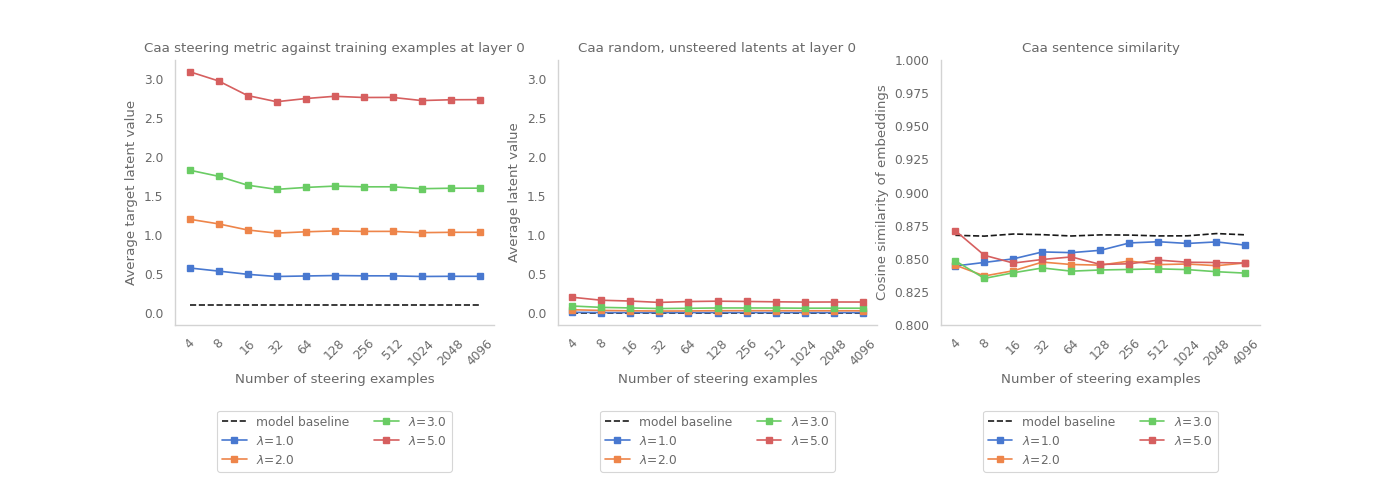
\includegraphics[width=\textwidth]{figures/gpt2_sweep_0.png}
        \label{fig:0}
\end{figure}

\begin{figure}
    \centering
        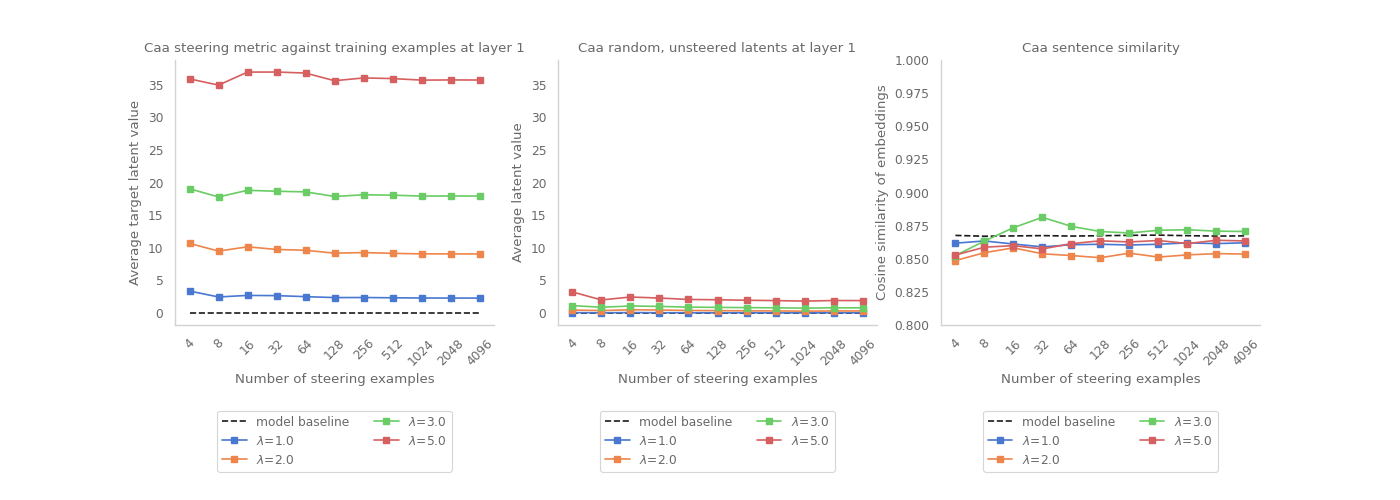
\includegraphics[width=\textwidth]{figures/gpt2_sweep_1.png}
        \label{fig:1}
\end{figure}

\begin{figure}
    \centering
        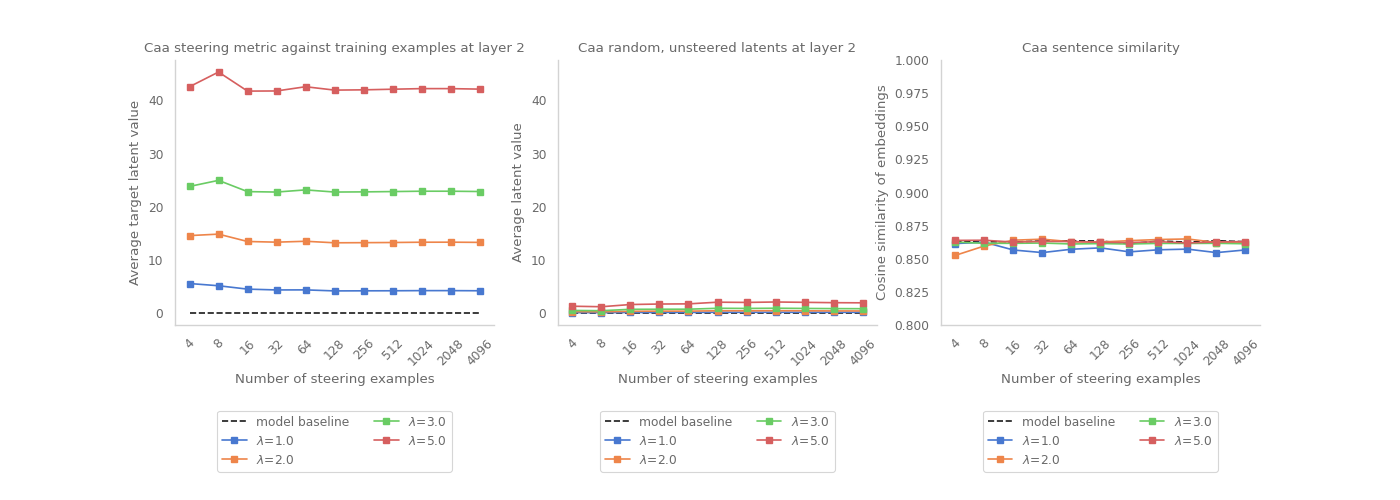
\includegraphics[width=\textwidth]{figures/gpt2_sweep_2.png}
        \label{fig:2}
\end{figure}

\begin{figure}
    \centering
        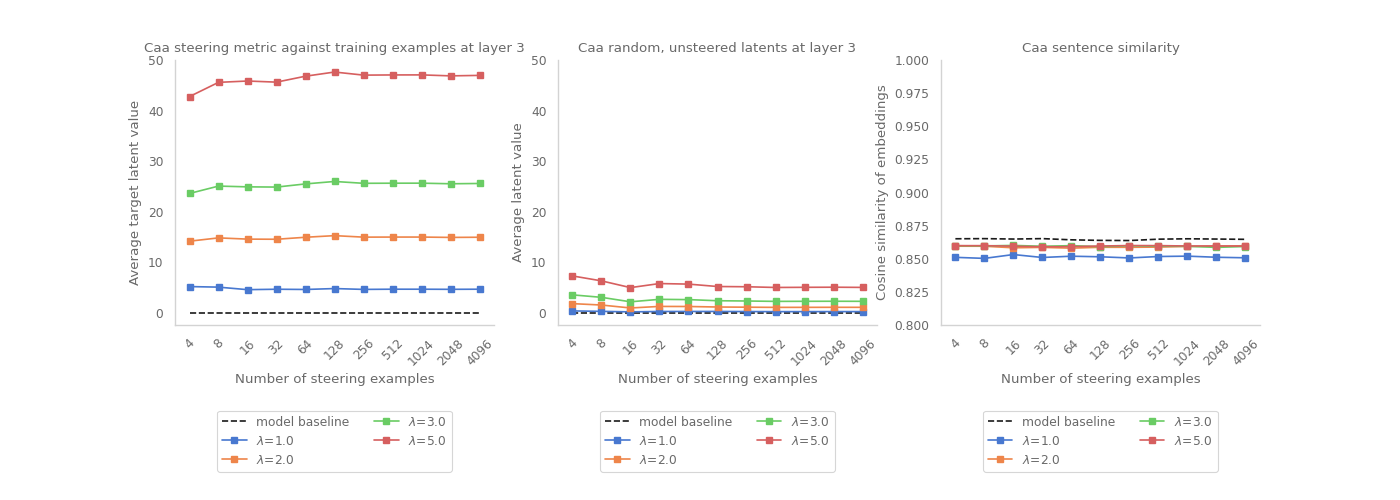
\includegraphics[width=\textwidth]{figures/gpt2_sweep_3.png}
        \label{fig:3}
\end{figure}

\begin{figure}
    \centering
        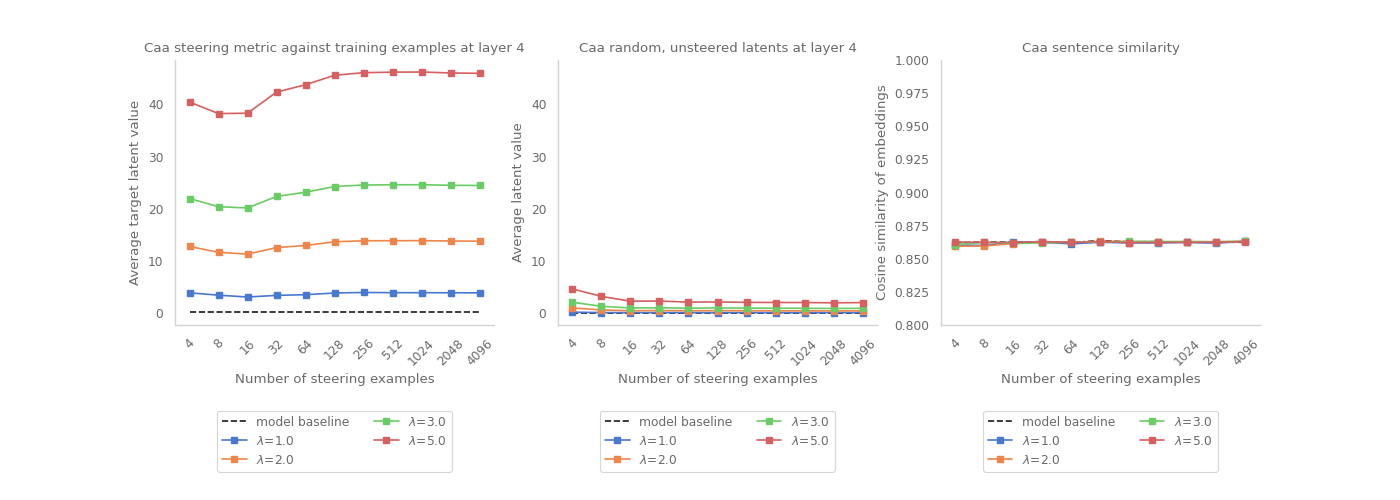
\includegraphics[width=\textwidth]{figures/gpt2_sweep_4.png}
        \label{fig:4}
\end{figure}

\begin{figure}
    \centering
        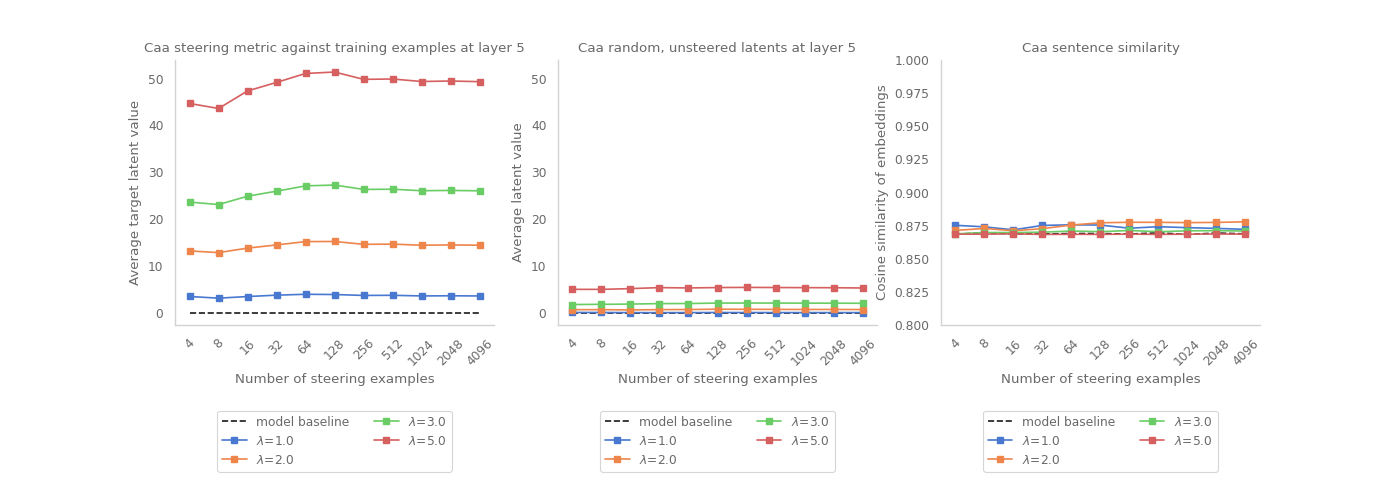
\includegraphics[width=\textwidth]{figures/gpt2_sweep_5.png}
        \label{fig:5}
\end{figure}

\begin{figure}
    \centering
        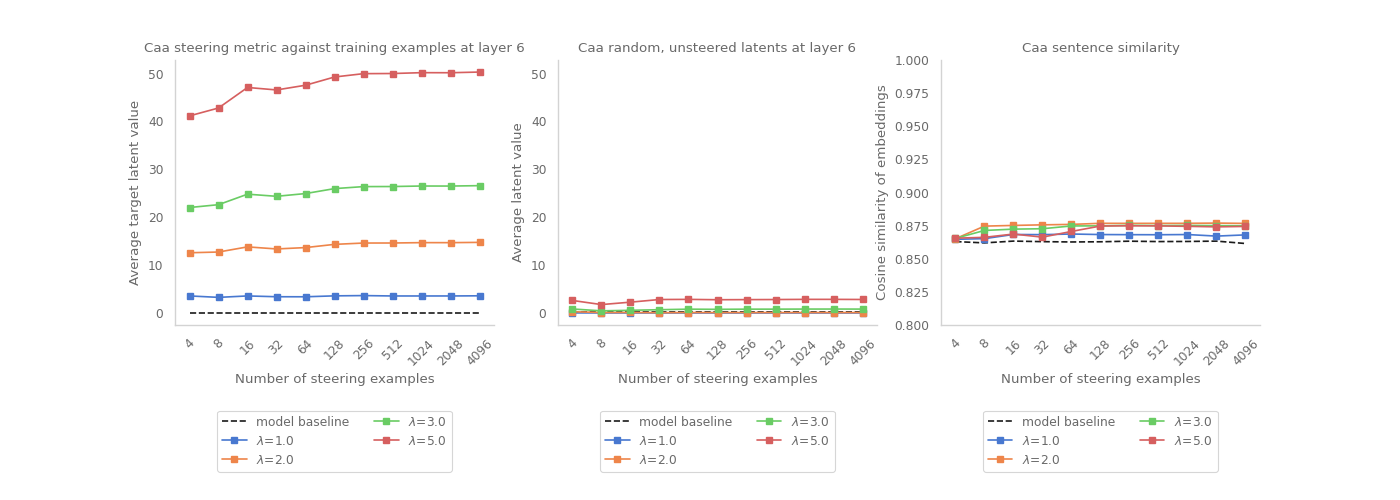
\includegraphics[width=\textwidth]{figures/gpt2_sweep_6.png}
        \label{fig:6}
\end{figure}

\begin{figure}
    \centering
        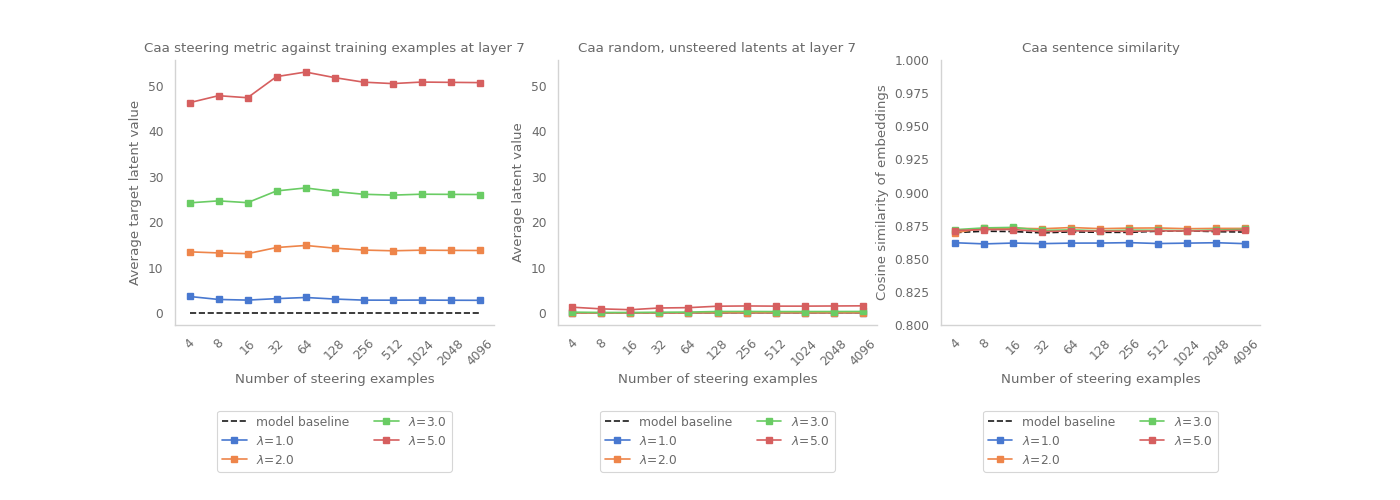
\includegraphics[width=\textwidth]{figures/gpt2_sweep_7.png}
        \label{fig:7}
\end{figure}

\begin{figure}
    \centering
    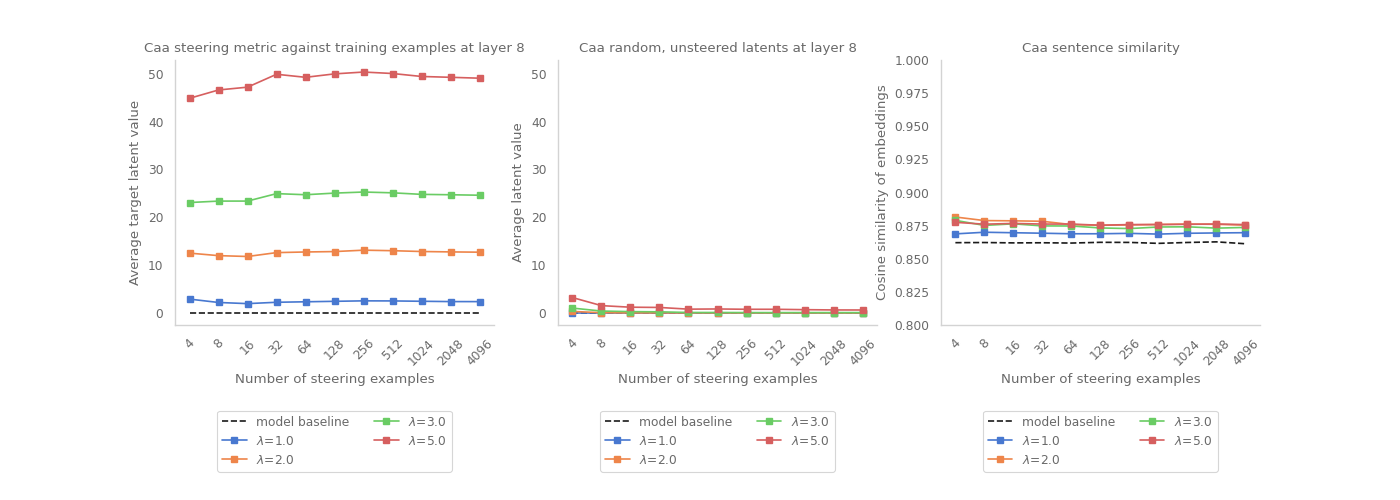
\includegraphics[width=\textwidth]{figures/gpt2_sweep_8.png}
    \label{fig:8}
\end{figure}

\begin{figure}
    \centering
        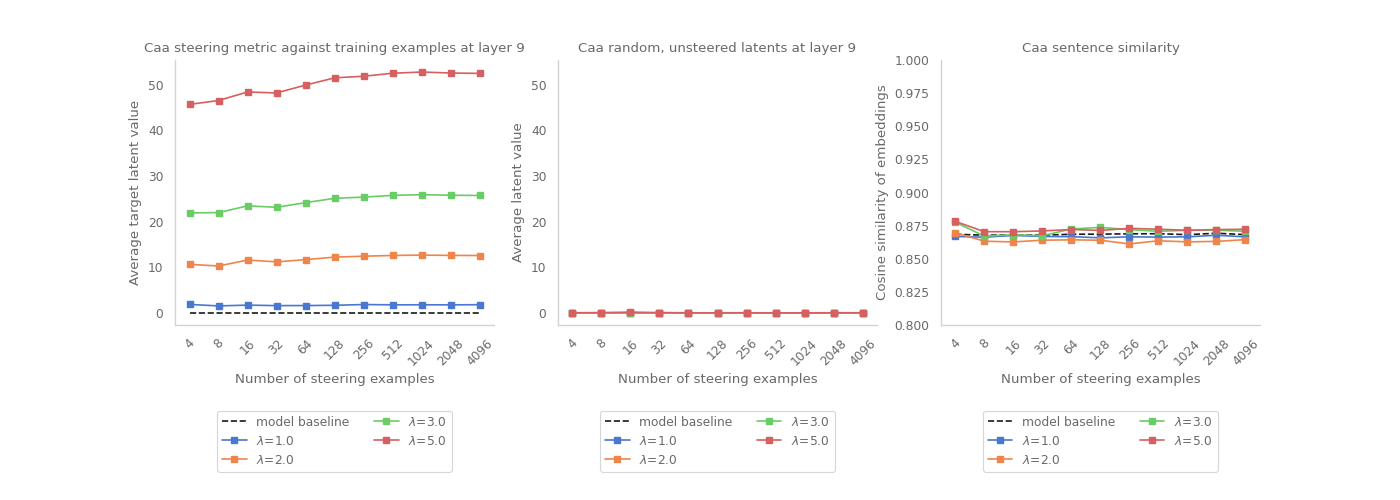
\includegraphics[width=\textwidth]{figures/gpt2_sweep_9.png}
        \label{fig:9}
\end{figure}

\begin{figure}
    \centering
        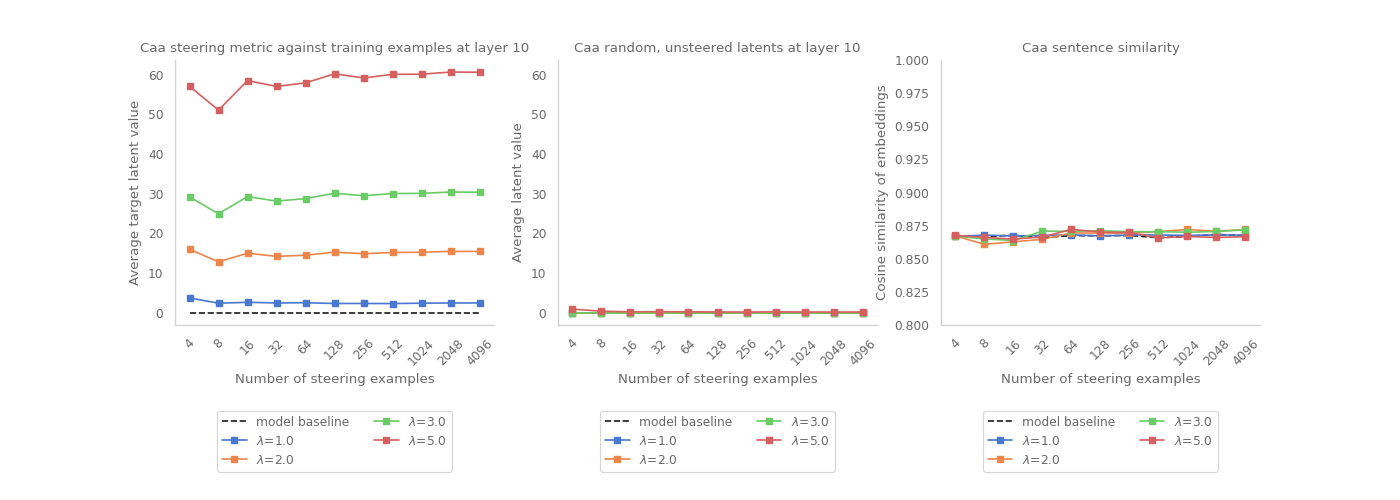
\includegraphics[width=\textwidth]{figures/gpt2_sweep_10.png}
        \label{fig:10}
\end{figure}

\begin{figure}
    \centering
    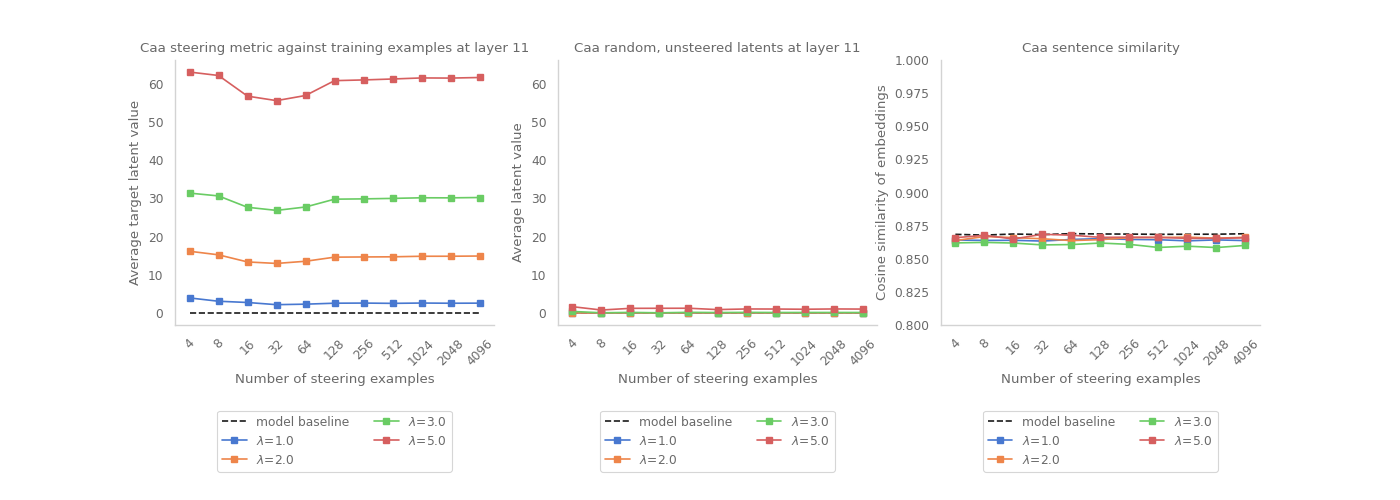
\includegraphics[width=\textwidth]{figures/gpt2_sweep_11.png}
    \label{fig:11}
\end{figure}
